
\documentclass{article}
\usepackage[utf8]{inputenc}
\usepackage[a4paper, total={7in, 8in}]{geometry}
\usepackage{braket}
\usepackage{xcolor}
\usepackage{amsmath}
\usepackage{amssymb}
\usepackage{amsfonts}
\usepackage{graphicx}
\usepackage{svg}
\usepackage{media9}
\usepackage{float}
\usepackage{tikz}
\usepackage[ruled,vlined]{algorithm2e}
\usepackage{pdfpages}
% \usepackage{biblatex} %Imports biblatex package
\usepackage{hyperref}
\usepackage{cleveref}
\hypersetup{colorlinks=true}

\usepackage[
backend=biber,
style=alphabetic,
sorting=ynt
]{biblatex}

\addbibresource{sample.bib} %Import the bibliography file

\newcommand{\commentt}[1]{\textcolor{blue}{ \textbf{[COMMENT]} #1}}
\newcommand{\ctt}[1]{\commentt{#1}}
\newcommand{\prb}[1]{ \mathbf{Pr} \left[ {#1} \right]}
\newcommand{\onotation}[1]{\(\mathcal{O} \left( {#1}  \right) \)}
\newcommand{\ona}[1]{\onotation{#1}}
\newcommand{\PSI}{{\ket{\psi}}}
\newcommand{\LESn}{\ket{\psi_n}}
\newcommand{\LESa}{\ket{\phi_n}}
\newcommand{\LESs}{\frac{1}{\sqrt{n}}\sum_{i}{\ket{\left(0^{i}10^{n-i}\right)^{n}}}}
\newcommand{\Hn}{\mathcal{H}_{n}}
% \author{David Ponarovsky}
% \date{July 2021}

\newcommand{\Ep}{\frac{1}{\sqrt{2^n}}\sum^{2^n}_{x}{ \ket{xx}}}
\newcommand{\HON}{\ket{\psi_{\text{honest}}}}
\usepackage{multicol}
% \usepackage{  }
\setlength{\columnsep}{0.6cm}


\begin{document}
    
\title{ Efficiently Trotterizing Lithium Time Eveloution Step  \\  Experimential Project  Classiq}
\author{David Ponarovsky}
\maketitle

\begin{abstract} 
In this paper, we review our experimental implementation of an algorithm for designing time evolution simulation circuits of molecules, given their Hamiltonian in the Pauli basis. Our algorithm employs several heuristics to minimize the circuit depth. We demonstrated this by taking the lithium molecule as a use case and comparing the generated circuit to the one produced by the naive approach.
\end{abstract}

\begin{multicols*}{2}

\section{Preamble.}
Simulation is definitely one of the core ingredients that our modern civilization relies on; the fact that one can check on their computer if their sketch for an electronic chip or plane will actually compute or fly without the need to construct and test a physical prototype both cheapens and accelerates the development process. 

Though humanity has successfully enabled an efficient simulation in a variety of regimes, there are still areas in which we don't have any other choice than to perform physical experiments. Development of materials, drugs, and medicines is a good example of a processes that suffer from the lack of simulation and can last for decades. What distinguishes those areas is the fact that the mechanics theory governing them is quantum mechanics, which we have good reason to believe cannot be simulated by classical computers. Yet, quantum computers are considered to be good candidates to overcome that barrier. 

Unfortunately, our current quantum machines are extremely limited in terms of computing resources; the most advanced computers have access to no more than a few hundred qubits and suffer from a considerable amount of noise, which cause long computations resulting in nonsense. Therefore, any short-term application must be cost-efficient.

On May 2022, Classiq, a pioneering quantum computing company, launched the first (at least at that scale) competition in quantum circuits programming. The initial purpose of this work was to solve the Lithium simulation problem. In short, the problem asked to come up with a quantum circuit, restricted to only a few qubits, that progress the lithium molecule in time. The winner of the competition would be the circuit with the shortest depth. We mention that our algorithm is generic and the software we have written can easily be modified for any other Hamiltonian.

The paper organized in the follow systematically manner, first in the preamble we will present the problem and talk about the general concepts which describe our specific Hamiltoinan, including the quantities regime (i.e number of qubits vs number of hamiltonians terms), the naive solution, and how mach improvement we could hope to make.     


Then in next section we review all the techniques that we have used to improve a  local gates assignment. Namely, this section deals with the question of how presenting each of the local term as subgate. 

  In contrast, the third and the forth sections reviews methods to determinate an  order which clearly superior comparing to the naive approach. The forth section presenting an concept of analyzing the "product graph" a concept which could be thought as the second order analyses of the alternate path from the third section.      
  \paragraph{The problem.} Generate a circuit, using no more than \(10\) qubits, that approximates the unitary \(e^{-iH}\) where \(H\) is the qubit Hamiltonian of a \textbf{LiH} (lithium hydride) molecule. The \textbf{LiH} Hamiltonian is composed of 276 Pauli strings, and can be found \hyperlink{LiH.html.pdf.1}{HERE}. The approximation error is defined in the next section, and should be less than \(0.1\). The circuit should be composed of the \(CX\) and single qubit gates only.

\paragraph{Naive approach.} Before diving into the technical details let's review our competitor first. Consider the straightforward assignment Lie-Trotter \cite{Lie-Trotter} just handle each of Hamiltonian terms one by one. Assume the the hamming weight of the support of \(H_i\) equal to \(d_i\). so we pay two steps to rotate each wire into the parity base and uncompute it in the end. then we could apply the \(CX\) from each qubit in the support to a chosen one which will sum the wires parity and finally will propgate the sum trough the \(RZ\left(\theta \Delta t \right) \) gate (rotation by the coefficient of the term and the step size). So in total we pay \((2 + 2d_i\) for each term and therefore the whole circuit will require: 

\begin{equation*}
    \begin{split}
        D^{\text{naive}}\left(n,m\right) & = \sum_{i}{2 + 2d_i} = m\sum_{i}{\frac{2 + 2d_i}{m}} = \\ & 2m \left\Big( 1 + \mathbb{E}_{\sim i}[H] \right\Big)  
    \end{split}
\end{equation*}

Where \( D^{\text{naive}}\left(n,m\right)\) is the depth of the circuit which compute a single \( \Delta t \) step of Lie-Trotter formula\cite{Lie-Trotter}. In order to getting a more solid feeling about what is good solution, let's assume for the moment that \( \mathbb{E}_{\sim i}[H] > 5 \), in that case we obtain that the naive approach obtain a circuit at depth \( \ge 2 \cdot 276 \cdot 6 \sim 3100 \). In the end we will see that our solution yields a \(1759\)-depth circuit. 

\paragraph{Characterize our \textbf{LiH}.} A native question that one might ask is whether exists a more efficient way to presents the Hamiltonian. So even we can't a sign that there is not, let's try to estimate how mach improvement can be achived by applying the Kitaev transformation. In one sentence, Kitaev has showed that the ladder and the annihilation operators has pauli representation such each operator touch at least \( \log\left(n\right) \) of the qubits. By the fact that Hamiltonian in the energy base has "product" of four operators (i.e \( a^{\dagger}_{i}b^{\dagger}_{j}a_{n}b_{m}) \) we get that there are might be operators in the computing base which touch \(4\log\left(n\right)\) qubits. In our case, \(n = 10 \Rightarrow 4\log\left(n\right) > n \). 
Bottom line, It seems that the known techniques for reducing asymptotically the support of the terms don't work here. Hence, it's also an hint that 10-factor improvement is unlikely. Therefore we will aim to 2-factor of improvement over the naive.    

\section{Single Term Heuristics.}

\paragraph{Main wire principle.} From now on we will call to the wire which sum the parity of the state the main wire. For given term we have chose the main wire to be the median of the wire in it's support. For example consider the following term:
\begin{equation*}
    XXXXIII
\end{equation*} 
Then as the second wire is above (and beanth) half of the wires, it will be the main wire in that case. the separation into upper and lower sides will enable to us to guarantee that at least two \(CX\) will be sum-up in parallel (using the next heuristic).
\paragraph{Upper and lower summations.}  We summing the parity as follow, denote by \( i_{1}, i_{2}, ... i_{W} , ... i_{k} \subset [n] \) the indices in the support of given term, such that \(i_{W}\) is the main wire. Then after rotate the wires into the phase base then we summing the parity of \(i_{1}, i_{2}, ... i_{W-1}\) into \(i_{W-1}\), That it, We apply a \(CX\left(i_{j}, i_{W-1}\right)\) for \(j < W-1\). 

As all the segements \([i_{j}, i_{W-1}]\) disjoint to any segments of the form  \([i_{W+1}, i_{j}]\) for \(j > W+1\) then we could sum the parity of \(i_{W+1},   i_{W+2} .. i_{k}\) wires into \(i_{W+1}\) in parallel. It's easy to see that this heuristic cut by almost half the depth of single term. 

\begin{figure}[H]
  \centering
    \includesvg[width = 280pt]{Ham_PRODUCT-2022-06-05 09:59:52.767380.svg}
    \caption{ Demonstration of the above methods, applied over the following terms    \( XIXZZXIXXZ \) \ \( XIXXZXIXXZ \). The fifth wire (qubit) is the main wire which sum the parity. }
    \label{fig:average-data-vs-model}
\end{figure}


\section{Greedy Order Heuristics.}
Next, we will review our methods to impose the gates order. Clearly the order does matter, to see that consider an hamiltonian pair which differ by only single coordinate i.e \(XXXX\) and \(XXXZ\). In that case the contribute of the first tree qubits remain the same for both of them, and therefore there is no needed to uncompute them after the applying of the first gate.      
\paragraph{Sample Greedy Diameters.} Assume that we given a set of therms with a promise that it might has a lot of "closer" terms (relative to the Hamming distance of their supports). Our first simple heuristic goal is to chain them together in greedy manner such that the distance of each adjacent terms will be minimal. 


\begin{algorithm}[H]
\SetAlgoLined
\ \\ 
\While { \( G \neq \empty \)  }{
\(T  \leftarrow\) Greedy Spanning Tree (\(G\)) \\
\(D_{i}  \leftarrow\) Diameter (\(T\)) \\
\(G \leftarrow G / D{i}\) \\
} 
\Return \(D_{0} ... D_{l}\) 
 \caption{Chain an Hamiltonian set }
\end{algorithm}
It's worth to note that replacing the Greedy Spanning Tree by MST (and the diameter by just the DFS scanning order of the MST) could be proving as 2-OPT in the terms of chaining. We think about the uncompute stage as the climbing back at the tree, and therefore \( \textbf{OPT} \le 2w\left(\text{MST} \right) \). But also it easy to see that every path which contain all the vertices has weigth greater than \(w\left(\text{MST} \right) \), Hence  \(2w\left(\text{MST} \right) \le 2\textbf{OPT}\).          
Yet, By the fact that we have already improved the naive solution at factor which close to \(\frac{1}{2}\) and by the intuition that the optimal depth is not very far from the naive (don't expect that \( D^{\text{naive}} \ge 4 \textbf{OPT} \) we decided to stick to the greedy construction, which in the next chapter will generalized to the product graph. 

\paragraph{Hyperplanes separation.} The cost of chaining pair of Hamiltonians isn't  a monotone function of their Hamming distance, for example consider the case of two terms which have not overlapping at all, i.e \( XXXXIIII \) and \(IIIIXXXX \) then it's clear that those two can be impose such they will be computed in parallel.   


\begin{figure}[H]
  \centering
    \includesvg[width = 260pt]{Ham_PRODUCT-2022-06-05 11:40:16.002860.svg}
    \caption{ Example for a case in which chaining terms with high distance reduce the depth of the circuit. Here the terms are : \(XIXZZIIIII \) \( XXXZIIIIII \) \( IIIIIIXXZX\) \( IIIIIIZIZX \). }
    \label{fig:average-data-vs-model}
\end{figure}

Technically we have separated those groups by follow, first we have sorted the term collection by the follow weight functions \(f,g\) such that:
\begin{equation*}
    \begin{split}
        f\left(H_{i}\right) &= \min {j : H_{j^{\prime}} = I \ \text{for } j^{\prime} > j } \\
        g\left(H_{i}\right) &= \max {j : H_{j^{\prime}} = I \ \text{for } j^{\prime} \le j }
    \end{split}
\end{equation*}    
And then we have matched pairs till we get into intersection.  
\section{The Product Graph.}
The main disadvantage of the last separation is that it doesn't take into a count any relation between terms which classified in the same side of the plane. The suggested solution: We will say that the pair \(H_i, H_j\) share a "solid product" if  \( f\left(H_{i}\right) \le g \left(H_{j}\right) \) where \(f,g\) defined above. We denote such relation by \(\left(H_i, H_j\right) \in \textbf{SP} \). Define the graph \(G^2 = \left(V\times V , E^{\prime}\right)\) where \(V\) is the set of the terms, to be: 
\begin{equation*}
    \begin{split}
        E^{\prime} &= \left\{ \left\{ (u,v),(w,z) \right\} : (u,v),(w,z),(u,z),(w,v) \in \textbf{SP} \right\}  \\
        w(e) &= w\left( \left\{ (u,v),(w,z) \right\} \right) = \max { w(u,w),w(v,z) }
    \end{split}
\end{equation*}
Note, that in the \(G^2\) path which pass through all the vertices contain an \(|V|\) copies of each term. Hence looking for spanning trees makes no sense. Therefore our diameters sampler will be more appropriate for that task (when we ensure that each sampled tree contains at most one copy of each term).          

Another advantage of this method that it can be easily generalize to scanning triples or higher orders by taking higher power of the graph, the main disadvantage is (of course) processing time.       

The final submission is a mixture of all the methods we have reviewed above.   

\printbibliography 
\end{multicols*}
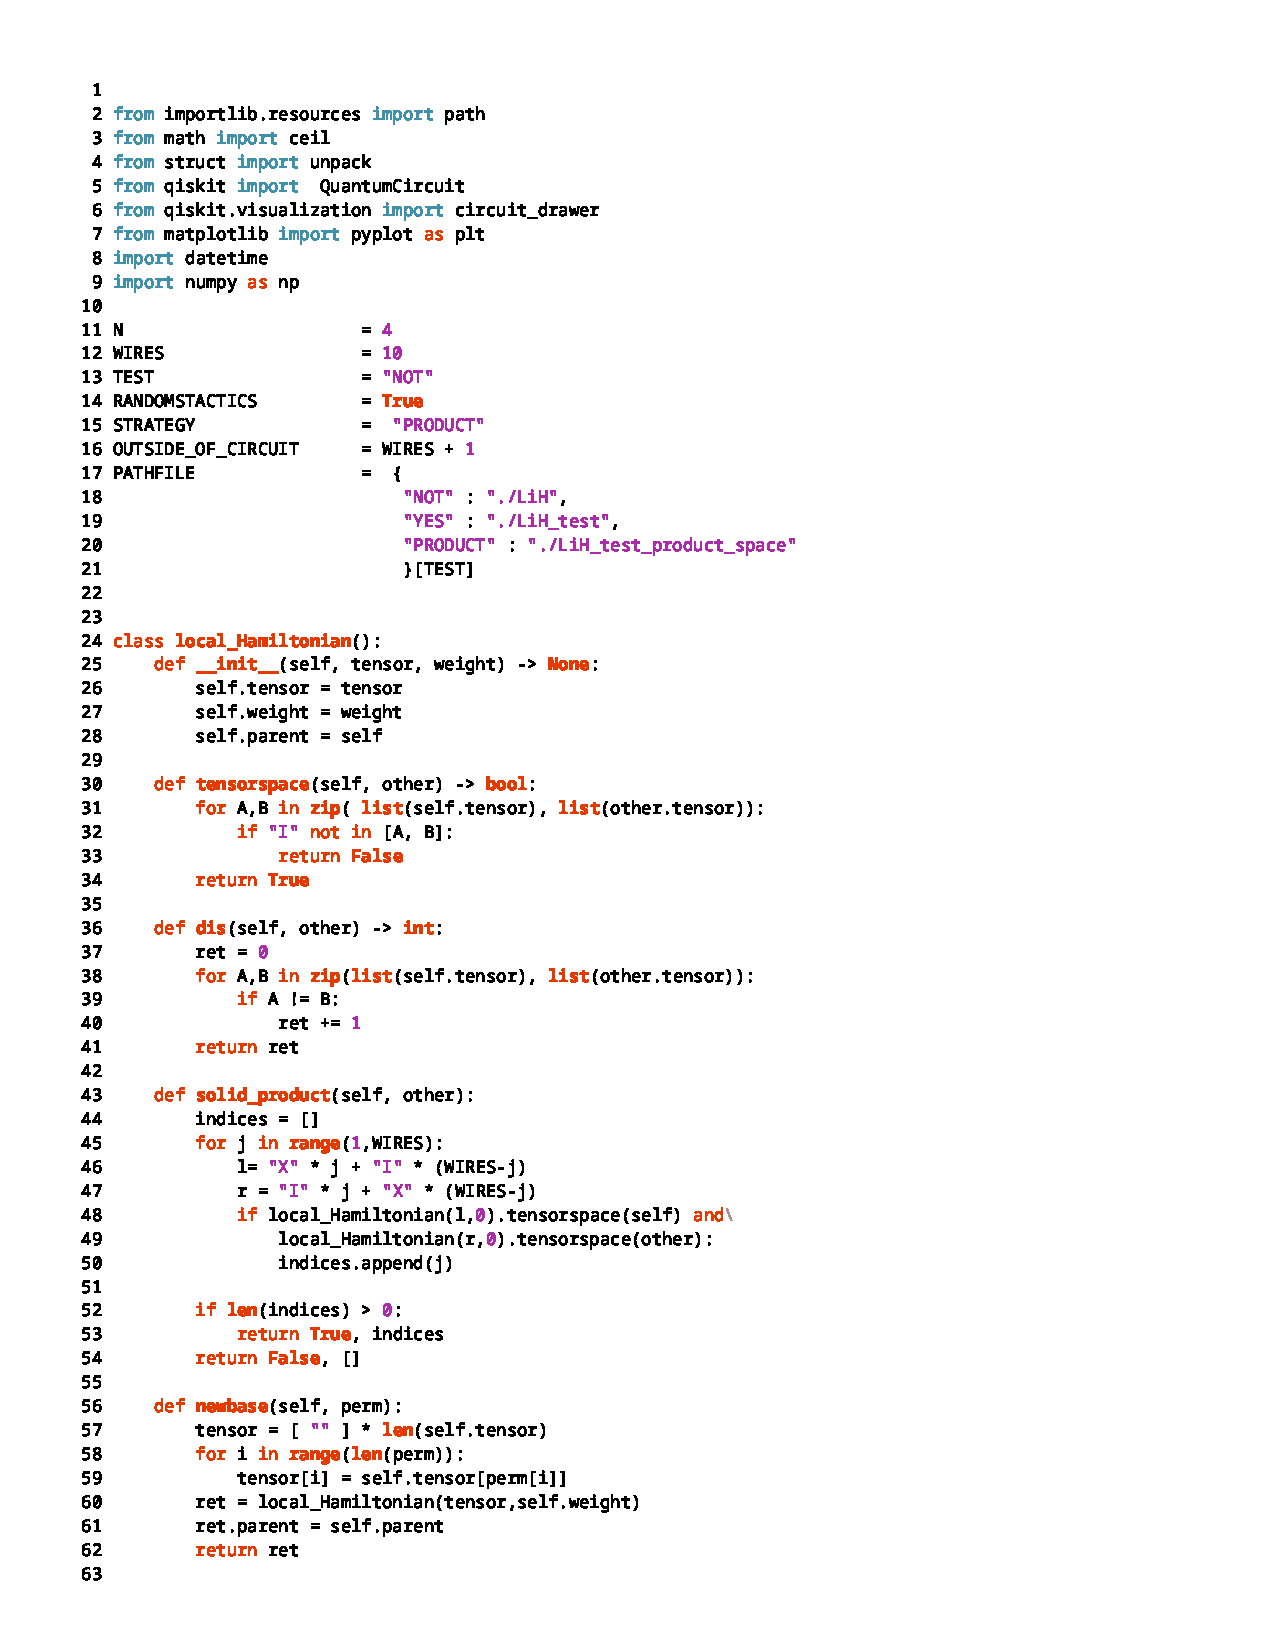
\includepdf[pages=-]{sourcecode.pdf}
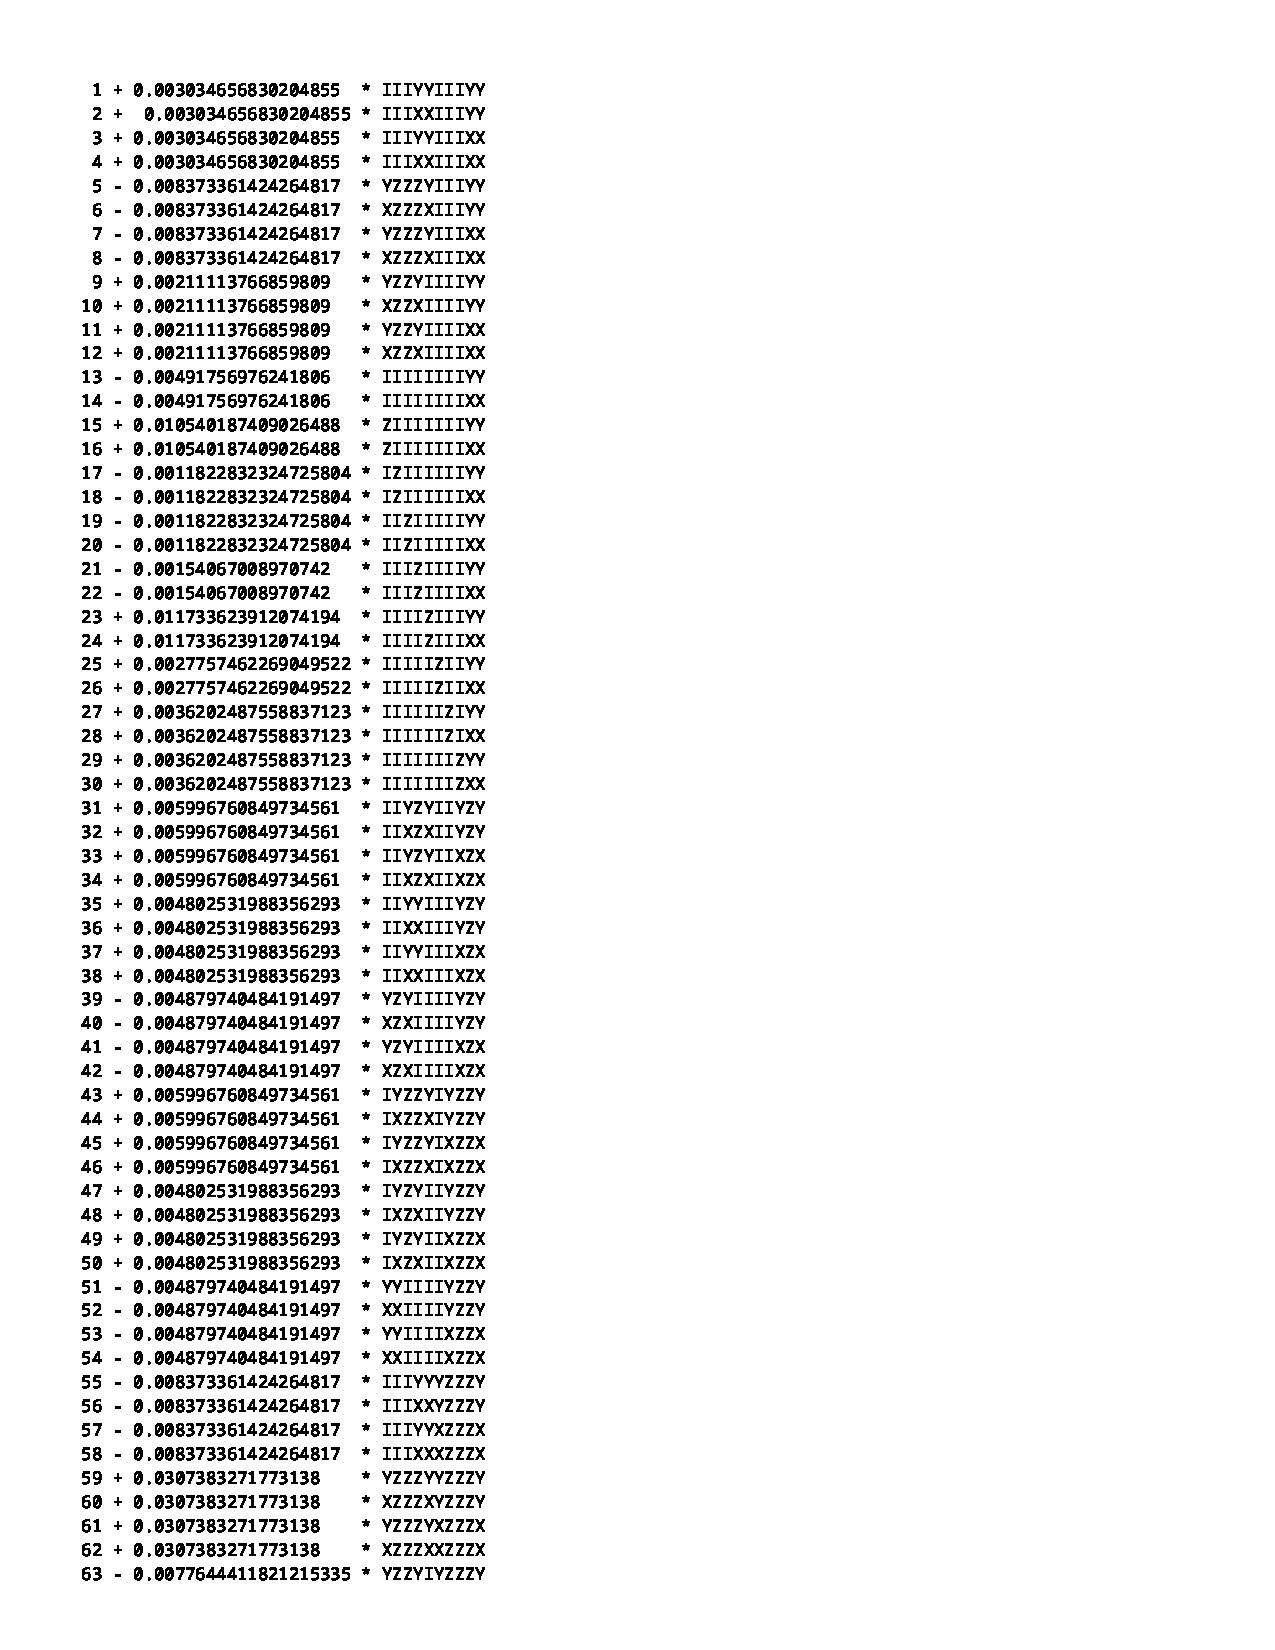
\includepdf[pages=-, link=true]{LiH.html.pdf}
\end{document}
